\section{Introduction}
The amount of blood in the human body can depend on a few factors, like your biological gender, how much do you weigh, and even where you live, but generally equivalent to 7\% of the body weight. The amount of blood in the human body can differ based on where you live. For example, people who live at higher altitudes usually have more blood because there isn’t as much oxygen as at the lower altitudes. The main component of the blood is plasma, which takes up to 55\% of it.
The plasma allows the blood to flow freely throughout the entire body inside blood vessels. Based on different attributes of the blood’s cellular components, like colour, size, texture, composition and shape, they are separated into three cell types: erythrocytes also known as Red Blood Cells (RBC), leukocytes (White Blood Cells or WBC short) and thrombocytes. Observing these molecules under the microscope, they have distinct shapes and sizes, WBCs being the larger ones due to the presence of nuclei and cytoplasm inside them. 
Based on these features WBC are further divided into two types: granulocytes and agranulocytes. 
Granulocytes are the most common WBC types defined by the granules inside their cytoplasm. The granulocytes, if dyed, can be categorized into four subtypes. These types differ in the colour of the granule stains inside the cytoplasm. The four cell types are neutrophils, eosinophils, basophils, and mast cells. The other type of WBC are agranulocytes that don't have granules in their cytoplasm and are further categorized into lymphocytes and monocytes.

\begin{figure}[htbp]
    \begin{center}
    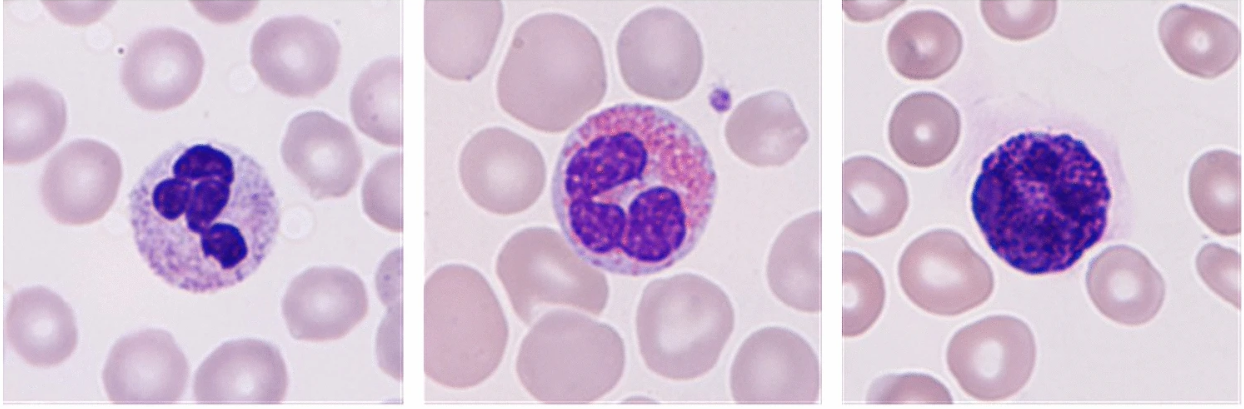
\includegraphics[scale=0.26]{wbc.png}
    \end{center}
    \caption{Three different types of WBCs: 1st: neutrophils, 2nd: eosinophils, 3rd: basophils}
    \label{wbc}
\end{figure}

A sample of 1 µl (= 0,001 ml) of human blood sample contains between 4000 and 11000 WBC. The distribution of different WBC types (Fig. \ref{wbc}) are the following: neutrophils between 40\% and 70\%, lymphocytes between 20\% and 45\%, monocytes between 2\% and 10\%, eosinophils between 1\% and 6\% and basophils under 1\%. Although basophils make up less than 1\% of the blood, they play an important role in the health of humans. Any minor imbalance might indicate serious health issues, e.g., leukemia,
\cite{AcuteLymphocyticLeukemia}
which has been considered as the leading death cause among various cancers due to lack of proper treatment. So it is important to diagnose the disease in the early stage. To avoid these kinds of diseases, it is necessary to determine the distribution and the exact count of WBC in the body. At the present there are two commonly used ways to achieve this: the first method involves a specialist who manually counts the cells with the help of a hemocytometer, while the other method is using an automated analyzer.
\cite{HemocytometerCounting}


Complete blood count
\cite{CBC}
is a blood analyzer which allows one to determine the count of the blood cells present in the body (Fig. \ref{wbc}). This allows the diagnosis of various disorders, for example, a lower WBC count than normal, called leukopenia, can forecast the presence of marrow cancer, autoimmune diseases, thyroid disorder, etc. A higher WBC count than normal can be a sign of a foreign substance present in the body. This is called leukocytosis and can cause several serious diseases like leukemia, marrow malformation, etc. In the treatment of these disorders, the key aspect is early diagnosis. In the treatment of leukemia early diagnosis greatly increases the chance of recovery, especially in children.



To achieve an early diagnosis, efficient and fast techniques are necessary so that the count and state of WBC can be determined to conclude results. 

There are several proposed methods to count WBCs that involve different Machine Learning (ML) techniques, mainly the usage of Convolutional Neural Networks(CNN). These CNNs are used to extract features. The proposed architectures combine multiple results of multiple CNNs to extract the features from the blood smear images. The features are then passed further in order to classify each blood cell.

The process of the classification of different blood cells from a smear image can be described with a few major steps. The first step is preprocessing the images, this often involves enhancement. CLAHE
\cite{CLAHE}
application on channels improves the contrast of a blood cell image. After preprocessing the images are prepared to be passed on to CNNs to extract the key features of the different cells on the images. The next step is feature selection. It is important because there can be several thousands of features and many of them may be redundant, inconsistent or irrelevant in the model construction. The last step is the creation of a classifier based on the extracted features beforehand. The model classifies the blood cell types, which then can be counted and analyzed.

The main contribution of this research is the modification and fine-tuning of an ML-based model involving multiple CNNs. In order to accelerate and decrease the computational needs, it proposes to decrement the number of selected features and replace the ResNet50 network. In cases, where the available data is imbalanced ResNet50V2 performs better, then ResNet50\cite{ResNet50V2Better}. The mentioned architecture uses a channel-wise CLAHE application to improve the contrast in the blood cell images. For feature extraction, it utilizes multiple CNNs, two already pre-existing Networks, namely ResNet50 and EfficientNetB0, and a network similar to AlexNet, named 4B-AdditionNet. For feature selections, it uses Ant Colony Optimization (ACO) and for classification, it uses multiple methods, like linear SVM (LSVM), Cubic SVM (CSVM), quadratic support vector machine (QSVM), linear discriminant analysis (LDA), fine K-nearest neighbour (FKNN), and coarse K-nearest neighbour (CKNN).
